%pme2360-ex
\section{Fator de Forma}
O fator de forma $F_{ij}$ é definido como \textit{ a fração da radiação que deixa a superfície i que é interceptada pela superfície j}. Considerando as superfícies $A_{i}$ e $A_{j}$ orientadas arbitrariamente conforme a figura \ref{fig:2}

% \begin{figure}[h]
% \begin{center}
% 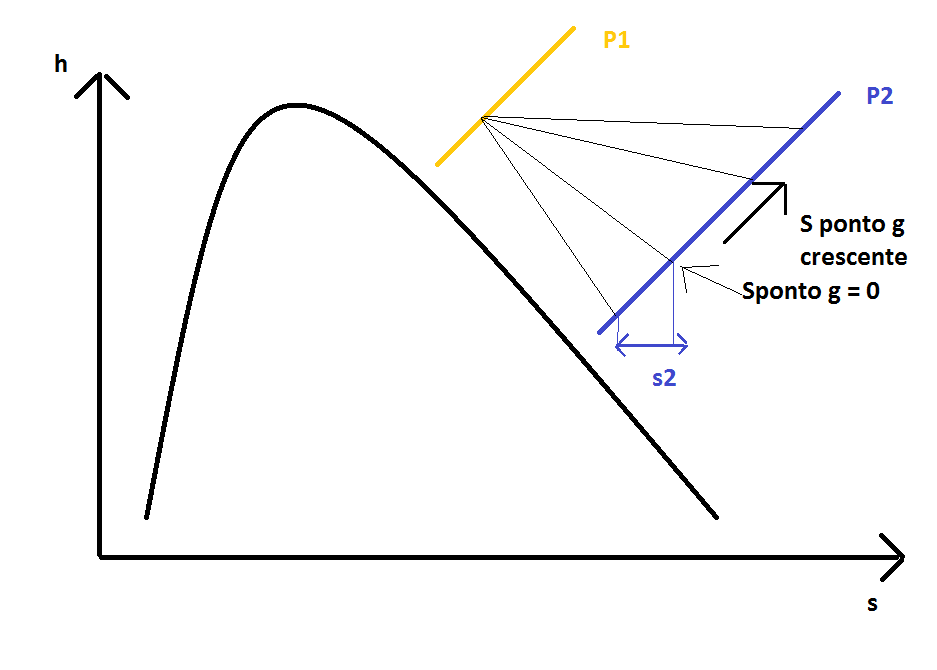
\includegraphics[scale=.35]{./fig/2.png}
% \caption{\label{fig:2}Fator de forma associado com a troca de radiação entre elementos de superfície de área $dA_{i}$ e $dA_{j}$}
% \end{center}
% \end{figure}

\myfig[scale=.35]{figPME2360-20111116-01e}{Fator de forma associado com a troca de radiação entre elementos de superfície de área $dA_{i}$ e $dA_{j}$}

Áreas elementares em cada superfície $dA_{i}$ e $dA_{j}$ são conectadas por uma reta de comprimento R, formando ângulos polares $\theta _{i}$ e $\theta _{j}$ com relação às normais $\textbf{n}_{i}$ e $\textbf{n}_{j}$. Os valores de R, $\theta _{i}$ e $\theta _{j}$ variam de acordo com as posições das áreas elementares $dA_{i}$ e $dA_{j}$.

A taxa na qual a radiaçao deixa $dA_{i}$ e é interceptada por $dA_{j}$ é definida como :

\[dq_{i \rightarrow j} = I_{i}\cos(\theta _{i})dA_{i}d\omega _{j-i}\]

Onde:
\begin{itemize}
\item $I_{i}$ é a intensidade da radiação que deixa a superfície $i$
\item $d\omega _{j-i}$ é o ângulo sólido subtendido por $dA_{j}$ visto de $dA_{i}$
\end{itemize}

Sendo $d\omega _{j-i}$ = ($\cos\theta_{i}\cos\theta_{j}$)/$R^{2}$, segue que:

\[dq_{i \rightarrow j} = I_{i}\frac{\cos\theta_{i}\cos\theta_{j}}{R^{2}}dA_{i}dA_{j} \]

Se a superfície \textit{i} emite e reflete difusamente ( $J = \pi I_{e+r}$), temos:

\[
	dq_{i \rightarrow j} = J_{i}\frac{\cos\theta_{i}\cos\theta_{j}}{\pi R^{2}}dA_{i}dA_{j} 
\]

A taxa total na qual a radiação deixa a superfície \textit{i} e é interceptada por \textit{j} é obtida, portanto, integrando-se sobre as duas superfícies:

\[
	q_{i \rightarrow j} = J_{i} \int _{A_{i}} \int _{A_{j}} \frac{\cos\theta_{i}\cos\theta_{j}}{\pi R^{2}}dA_{i}dA_{j} 
\] 

Onde $J_{i}$ é considerada uniforme sobre a superfície $A_{i}$.

Da definição de fator de forma como sendo a fração da radiaçao que deixa $A_{i}$ e chega em $A_{j}$:

\[F_{ij}=\frac{q_{i \rightarrow j}}{A_{i}J_{i}}\]

Temos que o fator de forma é definido por:

\[
	F_{ij} = \frac{1}{A_{i}} \int _{A_{i}} \int _{A_{j}} \frac{\cos\theta_{i}\cos\theta_{j}}{\pi R^{2}}dA_{i}dA_{j} 
\] 

\pagebreak

\section{Troca Radiante entre Superfícies}
Seja $q_{i}$ a taxa \textit{líquida} na qual a radiação deixa uma superfície $i$, representada por:

\begin{equation}
q_{i}=A_{i}(J_{i}-G_{i})
\label{eq:1}
\end{equation}

A irradiação da superfície $i$ pode ser calculada a partir das radiosidades de todas as superfícies no invólucro. Em particular, da definiçao de \textit{fator de forma}, a taxa total de radiação atingindo a superfície $i$ oriunda de todas as superfícies, incluindo $i$ é:

\[A_{i}G_{i}=\sum _{j=1}^{N}{F_{ji}A_{j}J_{j}}\]
Ou, usando a relação de reciprocidade, 

\begin{equation}
A_{i}G_{i}=\sum _{j=1}^{N}{A_{i}F_{ij}J_{j}}
\label{eq:2}
\end{equation}

Eliminando a área $A_{i}$ e substituindo \ref{eq:2} em \ref{eq:1}

\begin{equation}
q_{i}=A_{i}\left(  J_{i} - \sum _{j=1}^{N}{F_{ij}J_{j}}  \right)
\label{eq:3}
\end{equation}

Seja a relação da Regra do Somatório:

\begin{equation}
\sum _{j=1}^{N}{F_{ij}} = 1
\label{eq:4}
\end{equation}

De \ref{eq:4} em \ref{eq:3}:
\[
q_{i}=A_{i}\left(  \sum _{j=1}^{N}{F_{ij}}J_{i} - \sum _{j=1}^{N}{F_{ij}J_{j}}  \right)
\]
\\
Logo, usando a propriedade de linearidade da somatória

\begin{equation}
q_{i}=\sum _{j=1}^{N}{A_{i}F_{ij}(  J_{i} - J_{j}  )} = \sum _{j=1}^{N}q_{ij}
\label{eq:5}
\end{equation}

Ou seja, a taxa \textit{líquida} na qual a radiação deixa uma superfície $i$ equivale à soma das componentes $q_{ij}$ relativas à troca radiativa com outras superfícies. Fazendo uma analogia a um circuito elétrico com seus vários componentes (figura \ref{fig:1}), temos:

\begin{itemize}
\item ($J_{i}-J_{j}$) = potencial motriz
\item ($A_{i}F_{ij}$) = resistência espacial ou geométrica
\end{itemize}

% \begin{figure}[h]
% \begin{center}
% 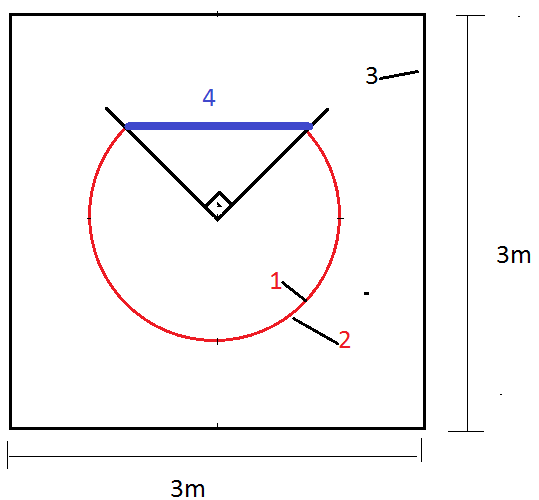
\includegraphics[scale=0.4]{./fig/1.png}
% \caption{\label{fig:1}representação do circuito equivalente}
% \end{center}
% \end{figure}

\myfig[scale=.4]{figPME2360-20111116-02e}{Representação do circuito equivalente}

Seja agora $q_{i}$ definida como:

\begin{equation}
q_{i}=\frac{E_{bi}-J_{i}}{(1-\varepsilon _{i})/\varepsilon _{i}A_{i}}
\label{eq:6}
\end{equation}

Em que $\varepsilon _{i}$ é a \textit{emissividade hemisférica total} da superfície $i$, $J_{i}$ é a \textit{radiosidade} da superfície, e $E_{b}$ o \textit{poder emissivo hemisférico total de um corpo negro}.

Combinando as equações \ref{eq:6} e \ref{eq:5}, temos:

\begin{equation}
\frac{E_{bi}-J_{i}}{(1-\varepsilon _{i})/ \varepsilon _{i}A_{i}} = \sum _{j=1}^{N} \frac{(  J_{i} - J_{j}  )} {(A_{i}F_{ij})^{-1}}
\label{eq:7}
\end{equation}

A equação \ref{eq:7} representa o balanço de radiação para o \textit{nó} da radiosidade associado com a superfície \textit{i} (figura \ref{fig:1}). E é especialmente útil quando a temperatura $T_{i}$ (e portanto $E_{bi}$) da superfície é conhecida.

\begin{equation}
q_{i} = \sum _{j=1}^{N} \frac{(  J_{i} - J_{j}  )} {(A_{i}F_{ij})^{-1}}
\label{eq:8}
\end{equation}

A equação \ref{eq:8} é especialmente importante quando a \textit{taxa de transferência líquida de radiação na superfície} é conhecida.